\documentclass[11pt,a4paper]{article}
\usepackage[utf8]{inputenc}
\usepackage[T1]{fontenc}
\usepackage{tgpagella}
\usepackage[spanish]{babel}
\usepackage{geometry}
\usepackage{booktabs}
\usepackage{xcolor}
\usepackage{titlesec}
\usepackage{fancyhdr}
\usepackage[parfill]{parskip}
\usepackage[expansion=false]{microtype}
\usepackage{hyperref}
\usepackage{setspace}
\usepackage{needspace}
\usepackage{graphicx}
\usepackage[table]{xcolor}
\usepackage{booktabs}
\usepackage{array}
\widowpenalty=10000
\clubpenalty=10000
\displaywidowpenalty=10000

\geometry{top=3.0cm,bottom=3.0cm,left=3.5cm,right=3.5cm}
\setlength{\parskip}{0.65em}
\setlength{\parindent}{0em}

\definecolor{azulai}{RGB}{30,80,140}
\definecolor{doradoai}{RGB}{140,90,0}
\definecolor{grisai}{RGB}{70,70,70}

\titleformat{\section}{\Large\bfseries\color{azulai}}{}{0em}{}[{\color{azulai}\titlerule[0.5pt]\nopagebreak[4]}]
\titlespacing*{\section}{0pt}{1.8em}{0.8em}
\titleformat{\subsection}{\large\bfseries\color{doradoai}}{}{0em}{}[{\nopagebreak[4]}]
\titlespacing*{\subsection}{0pt}{1.4em}{0.5em}
\titleformat{\subsubsection}{\normalsize\bfseries\color{grisai}}{}{0em}{}[{\nopagebreak[4]}]
\titlespacing*{\subsubsection}{0pt}{1.0em}{0.3em}

\pagestyle{fancy}\fancyhf{}
\rhead{\textcolor{grisai}{\small Virginia Riezu — Arquitectura Interna}}
\lhead{\textcolor{grisai}{\small Casas por signo}}
\cfoot{\textcolor{grisai}{\small\thepage}}
\renewcommand{\headrulewidth}{0.3pt}

\hypersetup{colorlinks=true,linkcolor=azulai,urlcolor=azulai}
\setstretch{1.45}
\tolerance=1500
\emergencystretch=4em

\begin{document}

% ── Portada ──────────────────────────────────────────────────────────────────
\begin{titlepage}
  \centering
  \vspace*{1.5cm}
  {\Huge\bfseries\color{azulai} Casas por signo}\\[0.5cm]
  {\large\color{grisai} Arquitectura Interna}\\[0.3cm]
  {\small\itshape\color{grisai} Organización de la vida: ejes, distribución e interceptaciones}\\[2cm]
  {\huge\color{doradoai} Virginia Riezu}\\[1.5cm]
  {\Large 06/09/1975 \quad 01:30}\\[0.3cm]
  {\Large Pamplona, España}\\[0.3cm]
  {\normalsize Lat: 42.8157° \quad Lon: -1.6522° \quad UTC+02:00}\\[0.3cm]
  {\normalsize Ascendente: Géminis 29°04' \quad
    MC: Piscis 3°22'}\\[2cm]
  \begin{tabular}{ll}
    \textbf{ASC (Casa 1):}  & Géminis 29°04' \\
    \textbf{DSC (Casa 7):}  & Sagitario 29°04' \\
    \textbf{MC (Casa 10):}  & Piscis 3°22' \\
    \textbf{IC (Casa 4):}   & Virgo 3°22' \\
  \end{tabular}\\[2cm]
  \vfill
  {\small Generado el 20/05/2026}
\end{titlepage}

\tableofcontents
\newpage

\begin{center}
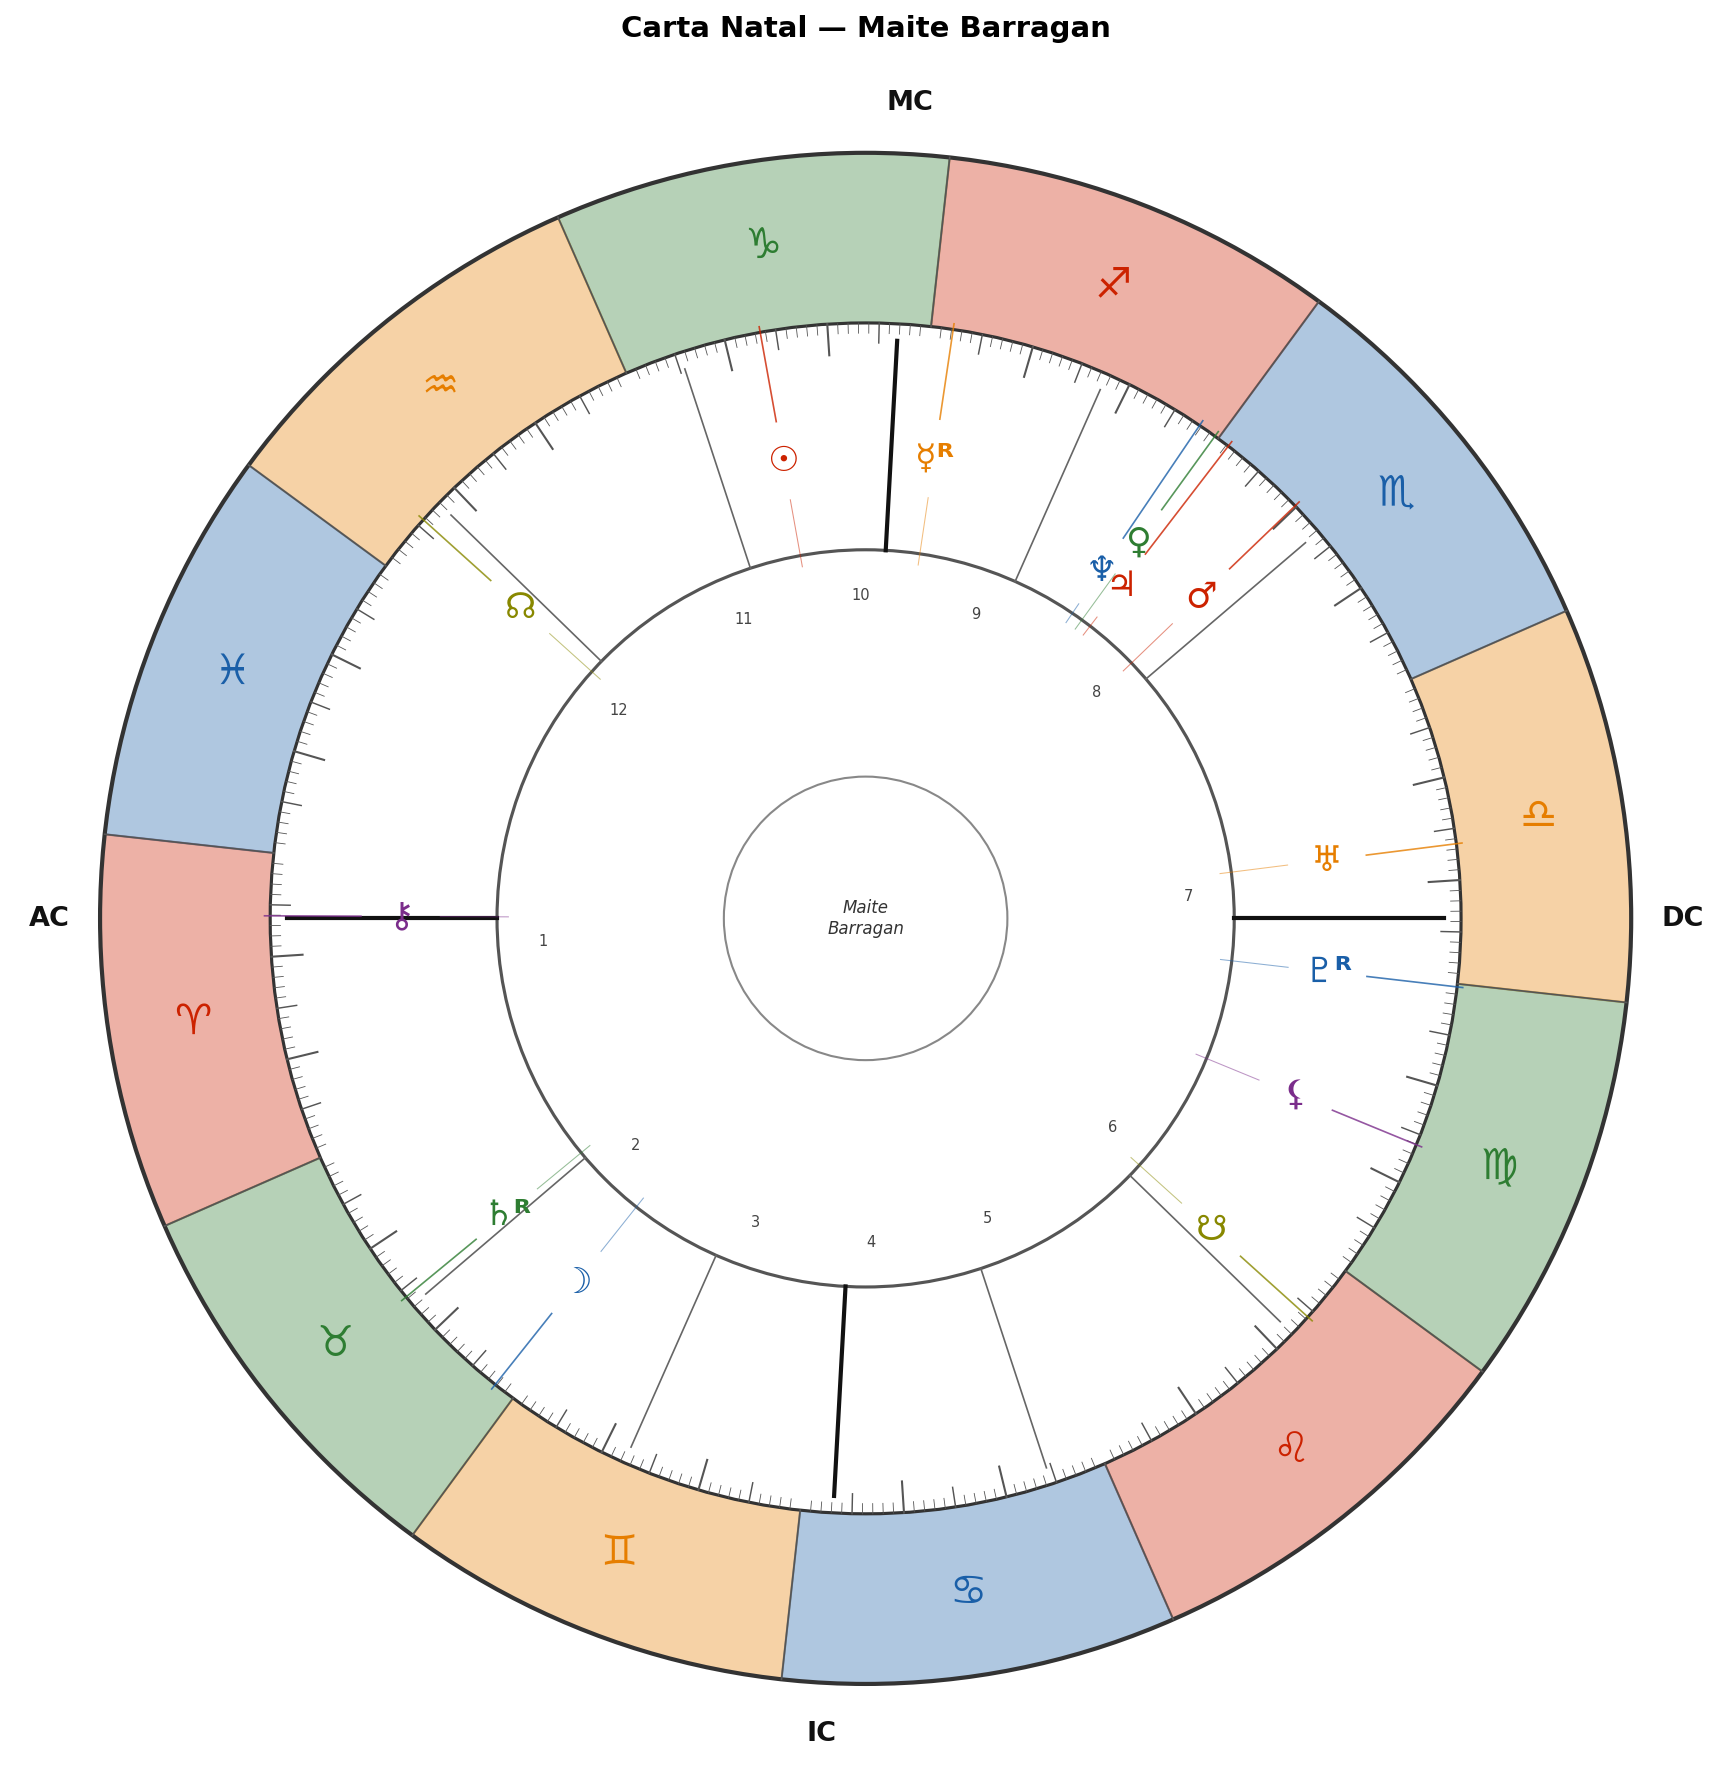
\includegraphics[width=0.88\textwidth]{rueda_casas.png}
\end{center}

\newpage

% ── Datos de referencia ───────────────────────────────────────────────────────
\section{Datos de referencia}

\begin{center}
\begin{tabular}{rllll}
  \toprule
  \textbf{Casa} & \textbf{Área} & \textbf{Signo} & \textbf{Cúspide} & \textbf{Planetas} \\
  \midrule
  1 & Identidad y presencia & Géminis & 29°04' & — \\
  2 & Recursos y seguridad & Cáncer & 18°32' & Saturno \\
  3 & Comunicación y entorno cercano & Leo & 8°44' & Venus \\
  4 & Base y hogar & Virgo & 3°22' & Sol, Luna \\
  5 & Expresión y creatividad & Libra & 6°39' & Mercurio, Urano, Plutón \\
  6 & Vida cotidiana y salud & Escorpio & 19°04' & Neptuno \\
  7 & Vínculos y relaciones & Sagitario & 29°04' & — \\
  8 & Transformación y profundidad & Capricornio & 18°32' & — \\
  9 & Horizonte y expansión & Acuario & 8°44' & — \\
  10 & Dirección y proyección & Piscis & 3°22' & — \\
  11 & Redes y colectivo & Aries & 6°39' & Júpiter \\
  12 & Mundo interior & Tauro & 19°04' & Marte \\
  \bottomrule
\end{tabular}
\end{center}

\vspace{0.3cm}\textit{No hay signos interceptados en esta carta.}

\newpage

% ── Interpretación ────────────────────────────────────────────────────────────
\section{Interpretación — Arquitectura Interna}

\begin{center}
{\small\itshape
No se trata de describir la personalidad.\\ Se trata de mostrar cómo está organizada la vida y qué implica esa organización.
}
\end{center}

\vspace{0.5cm}
\Needspace{5\baselineskip}

% ── 1. Estructura general ──────────────────────────────────────────────────────
\needspace{3\baselineskip}
\subsection{1. Estructura general de casas}

La mayor parte de los planetas principales (8 de 10) están en las casas 1–6. Esto suele indicar que buena parte de tu energía se orienta hacia la vida personal, el cuerpo, lo cotidiano y los procesos más íntimos antes que hacia la exposición pública.

La mayor parte de los planetas están en el sector oriental de la carta (casas 12–5: 8). Esto suele mostrar una vida más orientada por iniciativa propia, impulso interno y necesidad de decidir desde ti.

Casas con mayor concentración de planetas:
Casa 5 (Expresión y creatividad): Mercurio, Urano, Plutón — área especialmente importante
Casa 4 (Base y hogar): Sol, Luna — área con presencia relevante

Las casas con más planetas señalan áreas de vida donde se concentra mucha atención, movimiento interno y aprendizaje. No significa que sean las únicas importantes, pero sí que suelen tener más peso en tu manera de vivir, decidir y organizarte.

\vspace{0.5cm}
\Needspace{5\baselineskip}

% ── 2. Ejes principales ───────────────────────────────────────────────────────
\needspace{3\baselineskip}
\subsection{2. Ejes principales}

\subsubsection*{Ascendente — Géminis (29°04')}
Con Ascendente en Géminis, tiendes a entrar en la vida a través de la curiosidad, la comunicación y el intercambio con lo que te rodea. Sueles adaptarte rápido a los contextos y conectar fácilmente con distintas personas.

Las demás personas suelen percibirte como una persona ágil, cercana o fácil de tratar. A veces, sin embargo, puedes mostrar facetas muy distintas según el entorno y sentir que cuesta mantener una dirección completamente estable.

\subsubsection*{Descendente — Sagitario}
Con Descendente en Sagitario, tiendes a buscar relaciones donde exista crecimiento, libertad y apertura hacia algo más amplio. Necesitas sentir que el vínculo permite seguir expandiéndote.

Suele haber valoración de personas optimistas, abiertas o con ganas de explorar la vida, aunque a veces puede costar sostener relaciones demasiado cerradas o rutinarias.

\subsubsection*{Medio Cielo — Piscis (3°22')}
Con Medio Cielo en Piscis, sueles orientarte profesionalmente de forma sensible, intuitiva o difícil de encajar en estructuras demasiado rígidas. Muchas veces aparece necesidad de trabajar desde la inspiración, la creatividad o la conexión emocional.

Aquí suele haber capacidad de adaptación y percepción sutil, aunque a veces puede costarte definir límites claros o sostener una dirección profesional completamente estable.

\subsubsection*{Fondo del Cielo — Virgo}
Con Fondo del Cielo en Virgo, tu base interior suele sostenerse mejor cuando existe cierto orden, claridad y sensación de que las cosas están en su lugar. Muchas veces lo cotidiano influye muchísimo en cómo te sientes por dentro.

Aquí suele haber necesidad de organización y estabilidad práctica. Muchas veces recuperas energía cuando el entorno inmediato está cuidado y las pequeñas cosas funcionan con armonía.

\subsubsection*{La relación entre los ejes}
Ascendente (Géminis, Aire) y Medio Cielo (Piscis, Agua) están en elementos que pueden crear tensión. Puede haber diferencia entre cómo entras en las situaciones y lo que necesitas construir o mostrar hacia fuera. A veces esto hace que las demás personas perciban una parte de ti mientras tu dirección profunda va por otro lugar.

\vspace{0.5cm}
\Needspace{5\baselineskip}

% ── 3. Signos por casas ───────────────────────────────────────────────────────
\needspace{3\baselineskip}
\subsection{3. Distribución de signos por casas}

\subsubsection*{Casa 1 — Identidad y presencia · Géminis}
La Casa 1 habla de cómo entras en la vida y de la impresión que sueles generar de forma espontánea. Tiene relación con la presencia, el cuerpo y la manera en que tiendes a posicionarte cuando algo comienza.

Con Géminis en la cúspide, esta área suele vivirse desde la curiosidad, el movimiento y la necesidad de variedad. Tiendes a aprender rápido y a conectar fácilmente con distintas ideas o personas.

Aquí suele haber agilidad mental y facilidad para adaptarte, aunque mantener una única dirección durante mucho tiempo puede hacerse más difícil.

\subsubsection*{Casa 2 — Recursos y seguridad · Cáncer}
La Casa 2 muestra tu relación con la seguridad, los recursos y aquello que necesitas para sentir estabilidad. Aquí aparecen tanto lo material como la sensación interna de sostén.

Con Cáncer en la cúspide, esta parte de la vida suele vivirse de forma muy sensible y personal. Necesitas sentir seguridad emocional antes de abrirte o avanzar realmente en este ámbito.

Aquí tiene mucha importancia la protección, el cuidado y la sensación de pertenencia, aunque a veces puedes cerrarte si no sientes suficiente confianza.

Planetas en esta casa: Saturno. Este planeta añade una capa importante a la manera en que vives esta área.

\subsubsection*{Casa 3 — Comunicación y entorno cercano · Leo}
La Casa 3 se relaciona con la comunicación cotidiana, el pensamiento habitual y el entorno cercano. Habla de cómo procesas lo inmediato y de la manera en que intercambias información con lo que te rodea.

Con Leo en la cúspide, esta área suele cobrar fuerza cuando puedes expresarte con creatividad y sentir que lo que haces tiene valor o impacto. Suele haber bastante energía en este ámbito cuando puedes mostrarte con autenticidad.

Aquí puede aparecer necesidad de reconocimiento o de sentirte visto, aunque a veces el miedo a no recibir respuesta puede hacer que te retraigas más de lo que parece.

Planetas en esta casa: Venus. Este planeta añade una capa importante a la manera en que vives esta área.

\subsubsection*{Casa 4 — Base y hogar · Virgo}
La Casa 4 habla de la base emocional y del lugar interno desde el que necesitas sostenerte. Tiene relación con el hogar, las raíces, la intimidad y aquello que te ayuda a sentir refugio.

Con Virgo en la cúspide, esta área suele vivirse desde la observación, el detalle y la necesidad de mejorar las cosas poco a poco. Tiendes a fijarte fácilmente en lo que podría ajustarse o hacerse de una manera más precisa.

Aquí suele haber responsabilidad y atención práctica, aunque a veces puedes exigirte más de lo que realmente puedes sostener.

Planetas en esta casa: Sol, Luna. La presencia de varios planetas hace que esta área tenga mucho peso en tu carta. Suele ser un lugar donde se concentran aprendizajes, decisiones y movimiento interno.

\subsubsection*{Casa 5 — Expresión y creatividad · Libra}
La Casa 5 muestra cómo tiendes a expresarte cuando hay espacio para hacerlo libremente. Aquí aparece la creatividad, el disfrute, el impulso de crear y aquello que nace desde ti sin obligación.

Con Libra en la cúspide, esta área suele tomar forma a través de los vínculos y de la relación con otras personas. Necesitas cierto equilibrio o sensación de reciprocidad para sentirte bien aquí.

Aquí suele haber capacidad para dialogar, mediar o buscar armonía, aunque a veces puede costar tomar decisiones sin tener en cuenta constantemente a la otra persona.

Planetas en esta casa: Mercurio, Urano, Plutón. La presencia de varios planetas hace que esta área tenga mucho peso en tu carta. Suele ser un lugar donde se concentran aprendizajes, decisiones y movimiento interno.

\subsubsection*{Casa 6 — Vida cotidiana y salud · Escorpio}
La Casa 6 se relaciona con la vida cotidiana, los hábitos y la manera en que cuidas tu energía en el día a día. También habla de la relación con el trabajo cotidiano y con aquello que ayuda a sostener equilibrio y continuidad.

Con Escorpio en la cúspide, esta área suele vivirse con intensidad y profundidad. Suele haber dificultad para vivir superficialmente lo que ocurre aquí: cuando algo importa, suele implicar una implicación real.

Aquí suelen aparecer procesos de transformación importantes, aunque a veces también puede haber necesidad de control o dificultad para soltar.

Planetas en esta casa: Neptuno. Este planeta añade una capa importante a la manera en que vives esta área.

\subsubsection*{Casa 7 — Vínculos y relaciones · Sagitario}
La Casa 7 habla de los vínculos cercanos y de lo que aparece cuando entras en relación directa con otras personas. Aquí se desarrollan los acuerdos, las asociaciones y las dinámicas de espejo.

Con Sagitario en la cúspide, esta área necesita amplitud, sentido y sensación de crecimiento. Tiendes a moverte mejor cuando sientes que algo te abre horizonte o te permite avanzar más allá de lo conocido.

Aquí suele haber entusiasmo y necesidad de expansión, aunque a veces puede costar concretar o sostener todo lo que se inicia.

\subsubsection*{Casa 8 — Transformación y profundidad · Capricornio}
La Casa 8 se relaciona con los procesos profundos de cambio y transformación. Habla de lo compartido, de lo intenso y de aquello que suele remover capas internas importantes.

Con Capricornio en la cúspide, esta área suele vivirse con responsabilidad y visión a largo plazo. Tiendes a construir despacio, paso a paso, buscando resultados sólidos y duraderos.

Aquí suele haber constancia y capacidad de esfuerzo, aunque a veces puedes cargar con demasiado peso o sentir que nunca es suficiente.

\subsubsection*{Casa 9 — Horizonte y expansión · Acuario}
La Casa 9 muestra la necesidad de ampliar mirada y abrir horizonte. Tiene relación con el aprendizaje profundo, la búsqueda de sentido, los viajes y aquello que expande tu manera de comprender la vida.

Con Acuario en la cúspide, esta área suele vivirse de una manera distinta a la habitual. Necesitas libertad, espacio propio o una forma personal de hacer las cosas.

Aquí suele haber necesidad de independencia y mirada amplia, aunque a veces puede costar conectar con lo emocional o con lo más inmediato de este ámbito.

\subsubsection*{Casa 10 — Dirección y proyección · Piscis}
La Casa 10 habla de dirección, proyección y construcción visible. Aquí aparece la manera en que buscas desarrollar tu camino y el lugar que deseas ocupar hacia afuera.

Con Piscis en la cúspide, esta área suele vivirse de forma sensible, abierta y cambiante. Tiendes a percibir muchas capas a la vez y a dejarte afectar fácilmente por el ambiente o por lo que ocurre alrededor.

Aquí suele haber empatía, imaginación y capacidad de adaptación, aunque a veces puede costar poner límites claros o dar forma concreta a lo que sientes.

\subsubsection*{Casa 11 — Redes y colectivo · Aries}
La Casa 11 se relaciona con los grupos, las redes y los proyectos compartidos. Habla de cómo te vinculas con lo colectivo y de aquello que deseas construir junto a otras personas.

Con Aries en la cúspide, esta área de la vida suele moverse rápido. Tiendes a entrar antes de tenerlo todo claro y muchas veces necesitas descubrir sobre la marcha qué hacer con lo que aparece.

Aquí suele haber iniciativa, impulso y necesidad de avanzar, aunque a veces puede costar sostener lo empezado cuando desaparece la motivación inicial.

Planetas en esta casa: Júpiter. Este planeta añade una capa importante a la manera en que vives esta área.

\subsubsection*{Casa 12 — Mundo interior · Tauro}
La Casa 12 habla del mundo interior y de los procesos que necesitan silencio, retiro o más tiempo para poder comprenderse. Aquí aparecen muchas veces lo inconsciente, el descanso y las partes más difíciles de ver con claridad inmediata.

Con Tauro en la cúspide, esta parte de la vida necesita tiempo para asentarse. No sueles moverte deprisa aquí, pero cuando algo echa raíces puede mantenerse durante mucho tiempo.

La estabilidad tiene mucha importancia en este ámbito, aunque a veces puede costar hacer cambios incluso cuando ya serían necesarios.

Planetas en esta casa: Marte. Este planeta añade una capa importante a la manera en que vives esta área.



\vspace{0.5cm}
\Needspace{5\baselineskip}

% ── 4. Signos interceptados ───────────────────────────────────────────────────
\needspace{3\baselineskip}
\subsection{4. Signos interceptados}

\textit{No hay signos interceptados en esta carta. Los doce signos zodiacales están presentes en las cúspides de las doce casas.}


\vspace{0.5cm}
\Needspace{5\baselineskip}

% ── 5. Integración ────────────────────────────────────────────────────────────
\needspace{3\baselineskip}
\subsection{5. Integración}

Ascendente (Géminis, Aire) y Medio Cielo (Piscis, Agua) están en elementos que pueden crear tensión. Puede haber diferencia entre cómo entras en las situaciones y lo que necesitas construir o mostrar hacia fuera. A veces esto hace que las demás personas perciban una parte de ti mientras tu dirección profunda va por otro lugar.

La base interna (Virgo, IC) y la forma en que entras en la vida (Géminis, ASC) están en elementos que pueden crear tensión. Puede que lo que te sostiene por dentro no coincida del todo con la manera en que te muestras. Por eso puede ser importante darte tiempo para traducir lo interno hacia fuera sin forzarte a parecer de una forma que no respeta tu raíz.

La Casa 5 (Expresión y creatividad, Libra) concentra 3 planetas (Mercurio, Urano, Plutón). Esta área tiene mucho peso en tu carta y suele pedir atención especial. Cuando esta parte de la vida está cuidada, puede darte mucha fuerza. Cuando se carga demasiado, también puede absorber más energía de la que parece.

La Casa 4 (Base y hogar, Virgo) concentra 2 planetas (Sol, Luna). Esta área tiene mucho peso en tu carta y suele pedir atención especial. Cuando esta parte de la vida está cuidada, puede darte mucha fuerza. Cuando se carga demasiado, también puede absorber más energía de la que parece.

\vspace{0.5cm}
\Needspace{5\baselineskip}

% ── 6. Orientación práctica ───────────────────────────────────────────────────
\needspace{3\baselineskip}
\subsection{6. Orientación práctica}

\subsubsection*{Desde dónde empezar}
El área con mayor concentración es la Casa 5 (Expresión y creatividad, Libra). Puede ayudarte empezar por poner en palabras lo que ocurre y contrastarlo; nombrarlo puede darte claridad.

\subsubsection*{Qué estructurar primero}
La Casa 10 (Dirección y proyección, Piscis) muestra una parte importante de tu orientación hacia fuera. Lo primero que puede necesitar estructura aquí es cuidar el sostén emocional que necesitas para avanzar sin agotarte por dentro. Sin esa claridad, puede haber mucha energía disponible pero poca dirección de salida.

\subsubsection*{Qué evitar}
Conviene evitar exigirte que tu forma de presentarte (Géminis) y tu manera de construir dirección (Piscis) sean iguales. Son energías diferentes y pueden necesitar ritmos, decisiones y cuidados distintos.

\vspace{0.6cm}
Si no atiendes la distribución de las casas, las áreas más cargadas pueden absorber demasiada energía, mientras otras partes de la vida quedan poco cuidadas. La clave no es hacerlo todo con la misma intensidad, sino reconocer dónde hay más peso y qué zonas necesitan una atención más sencilla, clara y constante.

\vspace{0.5cm}
\Needspace{5\baselineskip}
\begin{center}
{\small\itshape\color{grisai}
La astrología se usa aquí como lenguaje simbólico de observación, no como definición de la persona.\\
El sistema es una aproximación funcional, no un diagnóstico.
}
\end{center}

\end{document}
